% --
% adversarial training

\section{Adversarial Pre-Training}\label{sec:exp_adv}
\thesisStateNotReady
Adversarial pre-training al already described in \rsec{nn_adv} is the transfer of learned weights obtained from adversarial training between a Generator (G) and a Discriminator (D) network.
The only neural network architecture used for adversarial pre-training is the \texttt{conv-jim} described in \rsec{nn_arch_cnn}.
To evaluate the gain of adversarial pre-training, the architecture is trained first with random init and compared to a training with adversarial pre-training. 
The training losses of those two training methods are shown in \rfig{exp_adv_fc3_train_loss} as well as their obtained accuracies in \rfig{exp_adv_fc3_val_acc}.

\begin{figure}[!ht]
  \centering
    \subfigure[adv init]{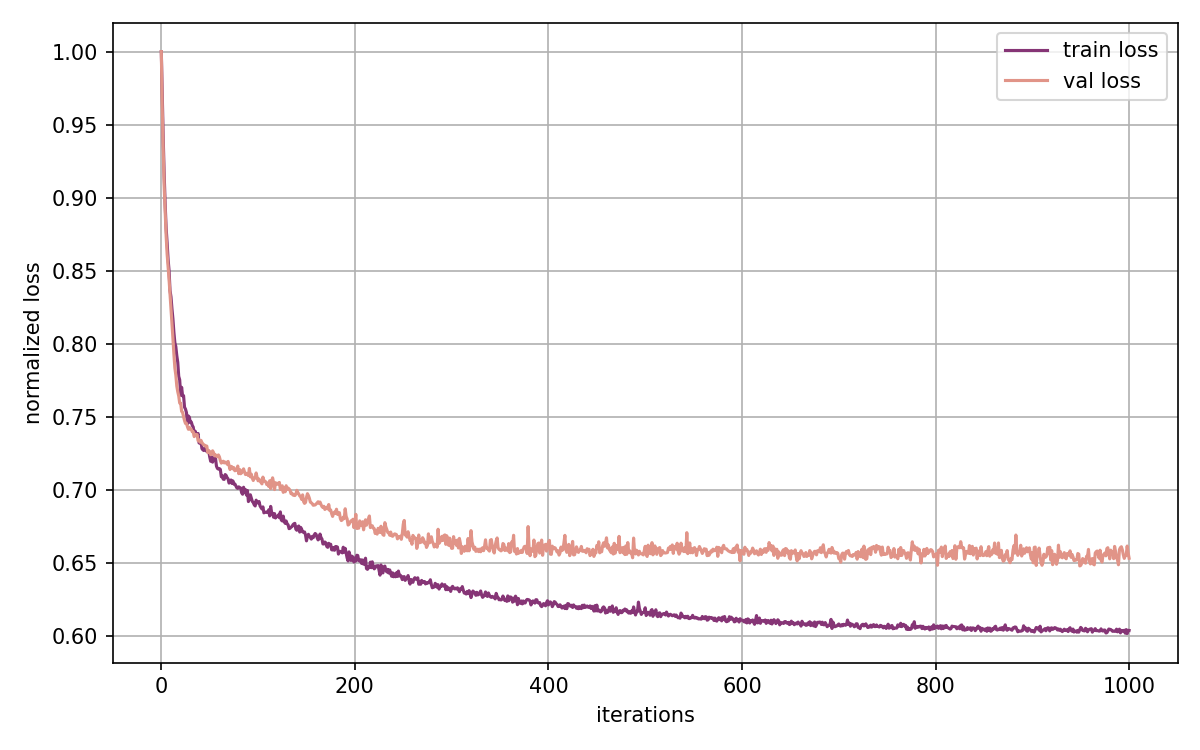
\includegraphics[width=0.45\textwidth]{./5_exp/figs/exp_adv_fc3_train_loss_label}}
    \subfigure[random init]{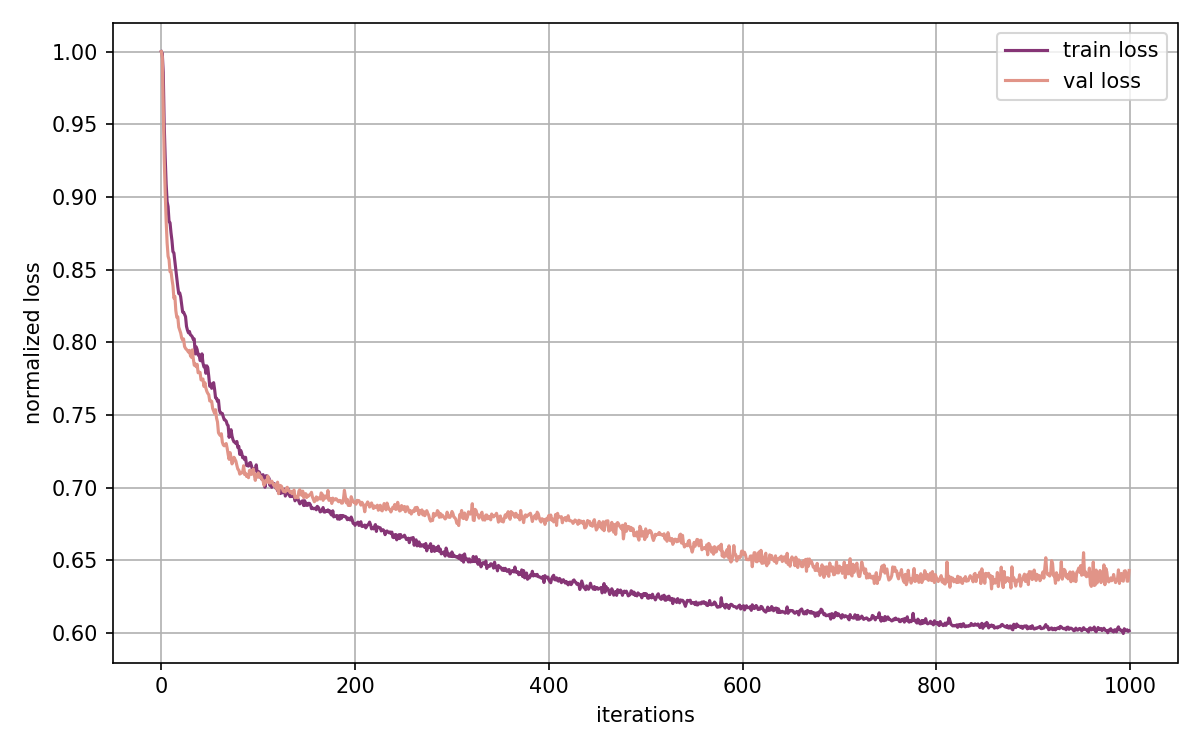
\includegraphics[width=0.45\textwidth]{./5_exp/figs/exp_adv_fc3_train_loss_random}}
  \caption{Comparing the train loss of L5-n500-norm1, c1d0dd0e0-norm1-it1000-bs32-lr0.0001-mo0.5 once with random init and once with adv init with dec-itl1000.}
  \label{fig:exp_adv_fc3_train_loss}
\end{figure}
\FloatBarrier
\noindent

\begin{figure}[!ht]
  \centering
    \subfigure[adv init]{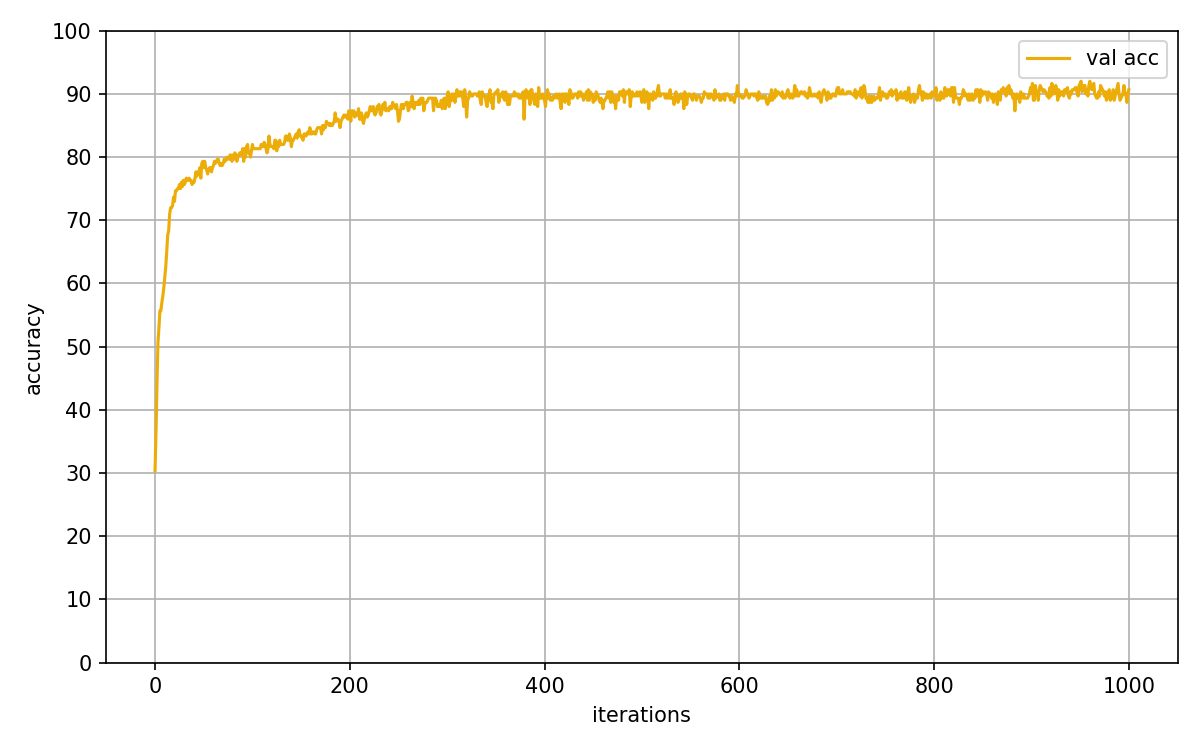
\includegraphics[width=0.45\textwidth]{./5_exp/figs/exp_adv_fc3_val_acc_label}}
    \subfigure[random init]{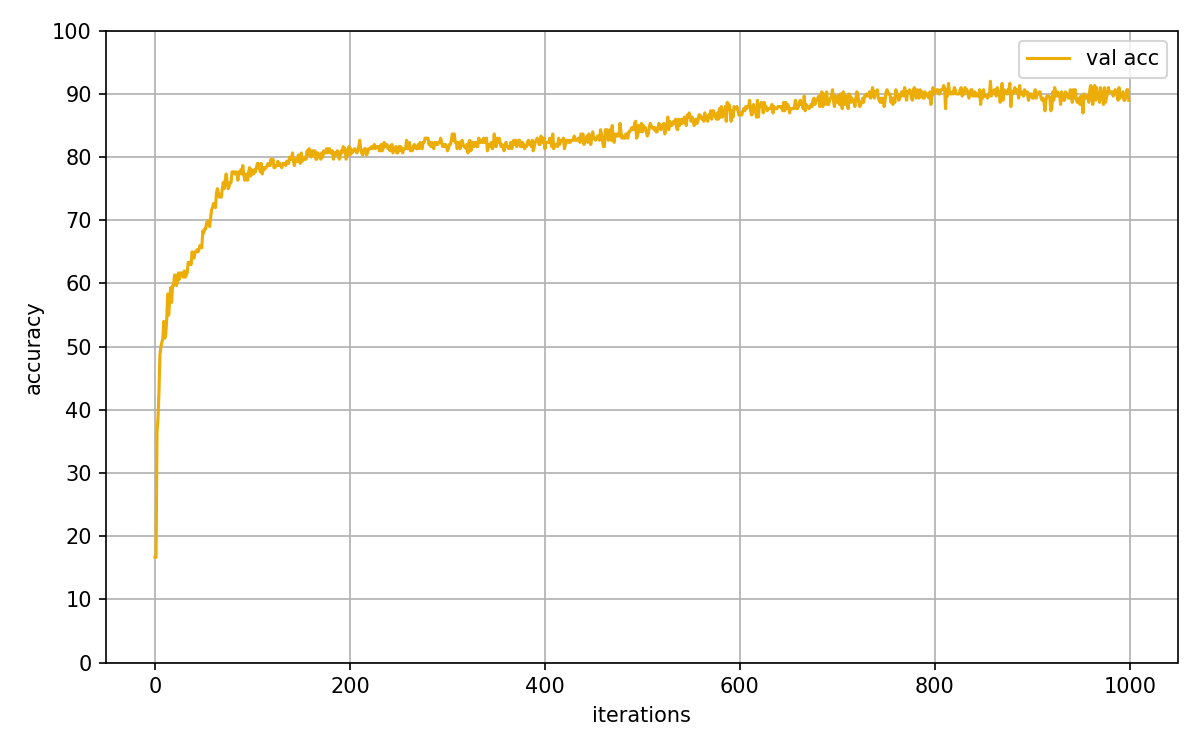
\includegraphics[width=0.45\textwidth]{./5_exp/figs/exp_adv_fc3_val_acc_random}}
  \caption{Comparing the validation accuracy of L5-n500, c1d0dd0e0-norm1-it1000-bs32-lr0.0001-mo0.5 once with random init and once with adv init with dec-itl1000.}
  \label{fig:exp_adv_fc3_val_acc}
\end{figure}
\FloatBarrier
\noindent

The loss and accuracy plots show how well the training was going forward for this showcase example. Both training work well and seem to converge, the one of the adversarial init parameters has a considerably faster convergence time here than the one without.
The scores on the test sets are shown in \rtab{exp_adv_fc3_score}, where both are achieving high scores on the test set, while the adversarial init one got a few percent more, but less on the my set.
This does not necessarily proof if one method is better or worse, therefore a more challenging task must be picked.
But at least it shows that adversarial pre training works at least as good as random initialization.
\begin{table}[ht!]
\begin{center}
\caption{Score comparison on arch: conv-encoder-fc3 with dataset: L5-n500 and training params: c1d0dd0e0-norm1-it1000-bs32-lr0.0001-mo0.5 and different adv params.}
\begin{tabular}{ M{2cm}  M{1.5cm}  M{1.5cm} }
\toprule
\textbf{adv params} & \textbf{acc test} & \textbf{acc my} \\
\midrule
none & 88.33 & 93.33 \\
dec-itl-1000 & 91.67 & 90.00 \\
\bottomrule
\label{tab:exp_adv_fc3_score}
\end{tabular}
\end{center}
\end{table}
\FloatBarrier
\noindent

